\subsection{Cross-Site Scripting (Weiland)}
Oft auch XSS genannt. Bei einem Angriff mit Cross-Site-Scripting wird eine Website, welche auch eine vertrauenswürdige Seite sein kann, vom Angreifer mit einem Script versehen, welches im Browser des Opfers ausgeführt wird.\\
Dabei muss der Angreifer nicht zwangsläufig auf den Server zugreifen können. Dadurch, dass viele Seiten dynamisch gestaltet sind, bieten sich einem Angreifer viele Möglichkeiten. Zum Beispiel gibt es oft die Möglichkeit eine Kommentar zu hinterlassen. Wenn in solch einem Feld ein Script platziert wird, wird es vom Browser eines Betrachters automatisch ausgeführt.
\paragraph{Problem}
Es gibt grundsätzlich drei verschiedene Arten von Cross-Site-Scripting:
\subparagraph{reflektiert oder nicht-persistent}
\subparagraph{persistent oder beständig}
\subparagraph{DOM-basiert oder lokal}
Der folgende Code (\autoref{lst:content_XSS_Vulnerable}) sollte eigentlich nur die mittels des GET-Parameter mitgegebene Eingabe ausgeben.
\begin{lstlisting}[style=custom, language=PHP, caption={Cross-Site-Scripting Anfällig},label={lst:content_XSS_Vulnerable}]
<html>
	<head>
	<title> Cross-Site-Scripting</title>
	</head>

	<body>
		<?php
		if(isset($_GET['input'])) echo $_GET['input'];
		else echo "keine Eingabe get&auml;tigt";			
		?>
	</body>
</html>
\end{lstlisting}

Wird diese Seite jedoch zum Beispiel mit dem GET-PArameter \texttt{input=<script type="text/javascript"> alert ('Dies sollte nicht passieren!') </script>} aufgerufen, wird das mitgegebene Script ausgeführt.


\paragraph{Methoden um Vorzubeugen}

Um XSS auf seiner eigenen Site zu verhindern sollten alle Eingaben, welche ausgegeben werden zum Beispiel mit dem Befehl \enquote{htmlspecialchars} behandelt werden. Dadurch werden alle Sonderzeichen durch die dafür vorgesehenen html-Zeichen umgewandelt (aus < wird \&lt;), wodurch kein ausführbares Script mehr vorliegt.

Manche Browser verhindern die Verwendung von XSS automatisch, so wird beispielsweise bei Internet Explorer 11 diese Meldung (\autoref{fig:content_security_xss_ie}) ausgegeben, wenn die Seite \autoref{lst:content_XSS_Vulnerable} mit einem Script als input aufgerufen wird.

\begin{figure}[H]
\centering
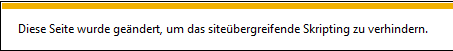
\includegraphics[keepaspectratio=true, width=14cm]{images/screenshots/xss_ie.png}
\caption{Internet Explorer blockiert XSS}
\label{fig:content_security_xss_ie}
\end{figure}